\documentclass[14pt]{extarticle}
\usepackage[utf8]{inputenc}

\usepackage{algorithm}
\usepackage{algpseudocode}

\usepackage{algpseudocode}
\usepackage{geometry}
\geometry{
    a4paper,
    left=30mm,
    right=10mm,
    bottom=20mm,
    top=20mm
}
\linespread{1.5}
\usepackage[english]{babel}
\usepackage{tempora}
\usepackage{newtxmath} 
\usepackage{ragged2e}
\usepackage{xparse}
\usepackage{indentfirst}
\usepackage{multirow}
\usepackage{tabularx}
\usepackage[table, x11names]{xcolor}
\usepackage{soul, color}
\usepackage{subfigure}
\usepackage{graphicx}
\usepackage{amsmath}
\usepackage{booktabs}
\usepackage[font=small]{caption}
\usepackage{algorithm}
\usepackage{subcaption}


\usepackage[
 bibstyle=gost-numeric-min,
% citestyle=gost-authoryear-min,
 citestyle=gost-numeric-min,
% citestyle=authoryear,
%    bibstyle=gost-numeric-min,
%  babel=other,
%  backend=biber,
% defernumbers=true,% Нумерация начинается как только встречается группа.
 sorting=none,
 url=false,
 doi=false,
 isbn=false,
 movenames=false,
 maxcitenames=2,
 maxbibnames=10
]{biblatex}


\let\openbox\relax
\usepackage{amsthm}
\addbibresource{ref/annot.bib}



\begin{document}
    \makeatletter
    \let\latexl@section\l@section
    \def\l@section#1#2{\begingroup\let\numberline\@gobble\latexl@section{#1}{#2}\endgroup}
    \makeatother
    
    \makeatletter
  \newcommand*\signaturelinewidth{5cm}
  \newcommand*\signaturelineheight{.4pt}
  \newcommand*\signaturedashleaderatom{\kern .1pt.\kern .1pt}
  \newcommand*\signaturelineraise{.4ex}
  \newcommand*\signaturelabelindent{.5cm}
  \newcommand*\signaturetextindent{}
  \newcommand{\llms}{LLMs}
  \newcommand{\llm}{LLM}
  \newcommand{\lora}{\textit{LoRA}}
  \newcommand{\dora}{\textit{DoRA}}
  \newcommand{\pissa}{\textit{PiSSA}}
  \newcommand{\adalora}{\textit{AdaLoRA}}
  \newcommand{\uidl}{\textit{UIDL}}
  \newcommand{\sleb}{\textit{SLEB}}
  \newcommand{\shortllama}{\textit{Shortened-LLaMA}}
  \newcommand{\ourmethodshort}{\textit{ID-LoRA}}
  \newcommand{\fullTuning}{FT}
  \newcommand{\peft}{PEFT}
  \newcommand{\gpt}{GPT2-M}
  \newcommand{\llamaTwoSmall}{LLaMA2-7B}
  \newcommand{\llamaTwoBig}{LLaMA2-13B}
  \newcommand{\qwenSmall}{Qwen2.5-3B}
  \newcommand{\qwenMedium}{Qwen2.5-7B}
  \newcommand{\qwenLarge}{Qwen2.5-32B}
  \newcommand{\eTwoENLG}{E2E-NLG}
  \newcommand{\alpaca}{Alpaca}
  \newcommand{\lisa}{\textit{LISA}}
  \newcommand{\ows}{\textit{OWS}}
  \newtheorem{definition}{Definition}

  \newcolumntype{t}{>{\centering\arraybackslash\hsize=.18\hsize}X}
  \newcolumntype{a}{>{\centering\arraybackslash\hsize=.17\hsize}X}
  \newcolumntype{T}{>{\centering\arraybackslash\hsize=.3\hsize}X}
  \newcolumntype{g}{>{\centering\arraybackslash\hsize=.09\hsize}X}
  \newcolumntype{M}{>{\raggedright\arraybackslash\hsize=.43\hsize}X}
  \newcolumntype{A}{>{\raggedright\arraybackslash\hsize=.32\hsize}X}
  \newcolumntype{S}{>{\raggedright\arraybackslash\hsize=.21\hsize}X}
  \newcolumntype{x}{>{\centering\arraybackslash\hsize=.41\hsize}X}
  \newcolumntype{z}{>{\centering\arraybackslash\hsize=.07\hsize}X}
  \newcolumntype{f}{>{\raggedright\arraybackslash\hsize=.19\hsize}X}
  \newcolumntype{u}{>{\centering\arraybackslash\hsize=.21\hsize}X}
  \newcolumntype{U}{>{\centering\arraybackslash\hsize=.23\hsize}X}
  \newcolumntype{F}{>{\raggedright\arraybackslash\hsize=.8\hsize}X}


  \NewDocumentCommand\signatureline{
    O{\signaturelinewidth}      % line width
    O{\signaturelabelindent}    % label margin
    O{%                           text indentation
      \ifx\@empty\signaturetextindent
        .5\dimexpr #2\relax
      \else
        \signaturetextindent
      \fi
    }
    m                           % label
    O{\signaturelineheight}     % line height
    O{\signaturelineraise}      % line raise
    D||{}                       % text
  }{%
    \parbox[t]{#1}{%
      \leftskip #3%
      \mbox{\strut #7}%
      \vskip -#6%
      \hrule height #5%
      \vskip #6%
      \scriptsize
      \leftskip #2%
      \rightskip #2%
      \strut #4%
    }%
  }
\makeatother


    \begin{titlepage}

    \begin{center}
        FEDERAL AUTONOMOUS EDUCATIONAL \\
        INSTITUTION OF HIGHER PROFESSIONAL 
        EDUCATION \\
        «NATIONAL RESEARCH UNIVERSITY \\
        «HIGHER SCHOOL OF ECONOMICS»
\\
\vspace{10mm}
        \textit {
            Faculty of Informatics, Mathematics, and Computer Science
        }
        \\
        \vspace{30mm}
        Novikova Irina Alekseevna \\
        \textbf{FINE-TUNING ACCELERATION OF LARGE LANGUAGE MODELS THROUGH THE LAYERWISE IMPORTANCE ANALYSIS}
        \vspace{1mm}
        \\
        \textit{Course work} \\
        \textit{in the field of \underline{01.04.02 Aplied Mathematics and Informatics}} \\

        educational program \\
        "Data Mining"\\
    \end{center}

\vspace{50mm}
\hfill
\begin{minipage}{0.4\textwidth}
    \begin{flushright}
        Academic Supervisor \\
        PhD in Computer Science \\
        % \signatureline[6cm]{}
        % \\
        A.V. Demidovskij
    \end{flushright}
\end{minipage}

\begin{center}
    \vspace*{\fill}
    Niznhy Novgorod, 2025
\end{center}

\end{titlepage}
    \setcounter{page}{2}
    
    \tableofcontents
    
\section*{Introduction}
\addcontentsline{toc}{section}{\protect\numberline{}Introduction}

    The \textbf{relevance} of this work is determined by the pivotal role that Large Language Models (LLMs) currently play in various domains including machine learning \cite{machine_learning}, computer vision \cite{computer_vision}, and natural language processing \cite{brown2020languagemodelsfewshotlearners}. These pre-trained LLMs are actively employed in numerous industrial applications, prized for their proficiency in tasks such as in-context learning \cite{brown2020languagemodelsfewshotlearners}, instruction following \cite{instruction_following}, and structured reasoning \cite{reasoning}. However, the capabilities of a pre-trained LLM may not be sufficient to tackle
    more specialized tasks, for example in medical or scientific domains. This necessitates extensive fine-tuning to tailor the models for specific downstream tasks. However, the fine-tuning process is extremely resource-consuming and demands signi-ficant
    memory and time resources resulting in low training throughput \cite{malladi2024finetuninglanguagemodelsjust}. This way, the evolvement of novel fine-tuning strategies that reduce time and memory costs without sacrificing model quality is of great importance.

    At the same time, given the vast parameter space of modern LLMs, which results in significant over-parameterization \cite{overparametrization}, identifying and leveraging the most essential model structures becomes crucial. These structures are vital as they disproportionately impact model performance \cite{yu2024superweightlargelanguage}. Effective utilisation of LLMs in various scenarios -- whether pre-training, fine-tuning, or inference -- demands a nuanced understanding of "importance" to discern these critical structures. This requirement extends across multiple optimization strategies including Neural Architecture Search \cite{LPZero} (NAS), \cite{synflow}, \cite{snip}, Parameter-Efficient Fine-Tuning (\peft{}) \cite{adalora}, \cite{lisa}, quantization \cite{quantization_1}, \cite{int8}, \cite{SqueezeLLM}, sparsification \cite{chess}, and model pruning \cite{uidl}, \cite{sleb}, \cite{wanda}. Each of these strategies aims to optimize different aspects of model architecture, yet they often rely on disparate heuristics for estimating importance, many of which lack general applicability or direct correlation with model quality \cite{LPZero}.

    This division highlights a glaring gap: the absence of a general methodology capable of assessing the importance of substructures across different \llm{} applications. Addressing this gap is not only crucial for enhancing model efficiency but also for advancing the methodologies used in model optimization, in particular, in the field of model fine-tuning acceleration. 

    The \textbf{practical significance} of this research is that it introduces a comprehensive overview of various existing importance estimation approaches as applied in distinct scenarios and presents a thorough examination of the most prominent approaches for importance analysis of Transformer blocks through the example of fine-tuning acceleration.

    The \textbf{novelty} of this work can be summarized as follows:
    \begin{itemize}
        \item This work introduces a comprehensive overview of existing methodologies for importance estimation of different structures, such as separate weights, layers, Transformer blocks, and even predicted architectures within the field of \llm{} across diverse application contexts. 
        \item This research provides evaluation of the most prominent approaches for esti-mating Transformer blocks importance within the context of accelerating the fine-tuning of \llms{}.
    \end{itemize}

    The \textbf{goal} of the present study is to accelerate the fine-tuning process by introducing the importance analysis of Transformer blocks within the \llm{}.

    To achieve the goal, the following \textbf{objectives} must be accomplished: 
    \begin{enumerate}
        \item Conduct comprehensive background study on the topic of fine-tuning \\ acceleration directions. 
        \item Provide an overview of existing methodologies for estimation the saliency of various structures within \llm{} in diverse application scenarios. 
        \item Conduct evaluation of the existing importance estimation techniques for \\ Transformer blocks in the context of accelerating the fine-tuning of \llm{}.
        \item Analyze obtained results and draw conclusion.
    \end{enumerate}

    The study employs a combination of \textbf{methodological approaches} to adress the research objectives. Firstly, it adopts a method of theoretical analysis and synthesis of existing literature to establish a solid theoretical foundation for the research. Secondly, programming methods are utilized to analyze the importance of \llms{}' Transdormer blcosk. Lastly, the study employs Deep Learning techniques to fine-tune \llms{}.

    The \textbf{object} of this study is the importance analysis of different structures within the \llm{}. The \textbf{subject} of the study is a thorough examination of the Transformer blocks-based importance approaches through the acceleration of fine-tuning process.

    This study was conducted as part of a \textbf{research project at the Huawei} dedicated to the fine-tuning acceleration of \llms{}.


    \section*{Chapter 1. Theoretical foundations of fine-tuning \\ acceleration through importance analysis}
\addcontentsline{toc}{section}{Chapter 1. Theoretical foundations of fine-tuning \\ acceleration through importance analysis}
\setcounter{section}{1}

    The goal of the present study is to develop a method for accelerating the fine-tuning of Large Language Models. However, the development of a novel approach requires a comprehensive analysis of existing techniques and promising ideas in this field, which can be leveraged in future work. This chapter is dedicated to such a thorough analysis and review.
    
    \subsection{Definition of Transformer-based architecture}
    Let $\mathcal{M}_\Phi$ represent an autoregressive Transformer model with parameters $\Phi \in \mathbb{R}^n$. The model $\mathcal{M}_\Phi$ is constructed as a sequence of Transformer blocks, denoted by $\tau$. Each layer $\tau_i$ is comprised of two main components: a Multi-Head Attention module (MHA) (\ref{eq:mha}) and a Feed-Forward Neural Network (FFNN) (\ref{eq:mlp}). For an input $x \in \mathbb{R}^n$, the MHA component utilizes $h$ parallel Attention heads to process the sequence.

    \begin{equation}\label{eq:mha}
    \begin{aligned}
        head_i & = Softmax(\frac{xW_q (xW_k)^T}{\sqrt{d_h}})xW_v \\
        MHA (X) & = Concat (head_1, \dots , head_h)W_o, 
    \end{aligned}
    \end{equation}
    where $i \in \mathbb{R}$, $W_o \in \mathbb{R}^{d \times d}$ is an output projection, and \(W_q, W_k, W_v \in \mathbb{R}^{d \times d_h}\) are query, key, and value projections of the $i$-th head; $d_h$ is typically set to $d/h$. 
    
    FFNN module consists of two linear transformations with an activation function (e.g. ReLU) (\ref{eq:mlp}). 

    \begin{equation}\label{eq:mlp}
        FFNN(x) = ReLU(xW_{up} + b_{up})W_{down} + b_{down}, 
    \end{equation}
    where $W_{up} \in \mathbb{R}^{d \times d}$ is the up-projection matrix and $W_{down} \in \mathbb{R}^{d \times d}$ is the down-projection matrix. 

    Within the \llm{} there exist a concept of the  \textit{importance} of certain structures. In this context, \textit{importance} facilitates the identification of structures that can be removed without affecting model performance. Thus, understanding the \textit{importance} of a structure helps assess its impact on the model's overall quality.

    Fine-tuning is the process of turning a general-purpose model into a specialized one while updating all pre-trained model parameters over a downstream task dataset. During the fine-tuning process \llm{} parameters are updated untill the loss function reaches approximately the optimum, indicating, that the model has been converged \cite{allenzhu2019convergencetheorydeeplearning} and is ready for deployment. 

    Assume that the data intended for fine-tuning is structured as a dataset $D = \{(x_i, y_i), i = 1, \ldots, N\}$, where $x_i$ represents an input sample and $y_i$ is the corresponding label; each $x_i$ and $y_i$ consists of sequences of tokens. The response produced by the model for $x_i$ is expressed as $\mathcal{M}_\Phi(x_i)$. It is presumed that the model has already been pre-trained, so its parameters are initially set to $\Phi_0$.

    Full fine-tuning involves altering these pre-trained parameters to $\Phi_0 + \Delta \Phi$, aiming to optimize the fine-tuning objective for $\mathcal{M}_\Phi$ with respect to $\Phi$, as given by (\ref{eq:full_fine_tuning}):
    \begin{equation}
        \label{eq:full_fine_tuning}
        \max_{\Phi} \sum_{(x, y) \in D} \sum_{t = 1}^{|y|} \log\left(\mathcal{M}_\Phi(y_t \mid x, y_{<t})\right),
    \end{equation}
    where $|y|$ denotes the number of tokens in the label sequence, and the dimensionality of $\Delta \Phi$ is the same as that of the initial parameter vector $\Phi_0$ \cite{lora}.
    
    The resources required for full fine-tuning of a model are comparable to those needed for pre-training an \llm{}; the only difference is that the full fine-tuning necessi-tates a smaller amount of a domain-specific data. Therefore, the development of approaches, that allow to reduce the number of required resources is of crucial importance. 
\subsection{Key directions in Large Language Models fine-tuning \\ acceleration}
    Several modern techniques have been developed to minimize the computational and memory demands associated with full fine-tuning. These approaches include reducing the training data volume (data reduction) \cite{aloe}, reducing the data precision (quantization) \cite{qlora}, reducing the number of parameters in an \llm{} (pruning) \cite{model_pruning}, eliminating resource-intensive backpropagation (backpropagation elimination) \cite{mezo}, \cite{hinton2022forwardforwardalgorithmpreliminaryinvestigations}, and leveraging Parameter-Efficient Fine-Tuning methods \cite{lora}.

    \subsubsection{Data reduction}
        Data reduction refers to the practice of removing less influential examples from a training set while aiming to preserve the \llm{} accuracy. This concept is generally realized through three main strategies: dataset distillation or condensation, coreset selection, and importance sampling, each offering a unique way to compress the training dataset.

        In dataset distillation, synthetic examples are generated based on statistical characteristics extracted from the original data \cite{cazenavette2022datasetdistillationmatchingtraining}. This strategy seeks to replace the full dataset with a much smaller, yet still representative, set of artificial samples that embody the key data patterns. Coreset selection, on the other hand, involves heuristics-based identification and selection of a crucial subset from the initial dataset \cite{shim2021coresetsamplingefficientneural}, ensuring that essential samples are retained and training efficiency is enhanced. Importance sampling deals with prioritizing those samples which are expected to have the greatest impact on model learning, primarily by focusing on instances that cause significant parameter updates during training \cite{jiang2019acceleratingdeeplearningfocusing}. For instance, ALOE \cite{aloe} prunes data points according to their loss values, evaluated by a trained or pre-trained model, achieving on average up to 33\% faster fine-tuning with a quality drop of 1.5\% compared to \lora{}. However, these data reduction strategies introduce additional computational cost, as they require a complete forward pass through the dataset to estimate the importance of each sample \cite{NEURIPS2018_967990de}.  

    \subsubsection{Quantization}
        Quantization refers to the process of converting data with high numerical precision into a format with lower precision. Although this method is primarily employed to speed up inference tasks, recent research has investigated its potential to also make fine-tuning processes more efficient.

        A prominent example is QLoRA \cite{qlora}, which leverages a 4-bit NormalFloat format to store the static, pre-trained language model. Meanwhile, essential computational tasks -- such as matrix multiplications involving \lora{} adapters -- are performed using 16-bit BrainFloat precision. While this strategy significantly reduces memory requirements, it tends to be slower than the traditional \lora{} approach, owing to the overhead of quantizing and dequantizing \llm{} parameters. Furthermore, applying extremely low-bit quantization may introduce substantial quantization errors, which can negatively affect the initial phase of \lora{} fine-tuning \cite{han2024parameterefficientfinetuninglargemodels}. Another technique, PEQA \cite{peqa}, adjusts the quantization scales of quantized \llm{} while keeping the integer matrices intact. Although this can cut memory usage by up to 92\%, it often comes at the cost of a notable drop in model quality, around 5\% compared to \lora{}. AlphaTuning is yet another method that involves quantizing a pre-trained \llm{} and perform selective fine-tuning of certain quantized parameters for targeted tasks \cite{AlphaTuning}. This approach achieves a 38\% acceleration in fine-tuning and reduces memory consumption by 80\%, but with a minimum quality reduction of 5\%.
    \subsubsection{Pruning}
        Model pruning is a technique aimed at reducing the model by eliminating redund-ant parameters or substructures. This process is primarily categorized into three approaches: unstructured, semi-structured, and structured pruning \cite{model_pruning}.

        Unstructured pruning removes individual parameters based on importance crite-rion, achieving high theoretical sparsity and minimal quality degradation. SOTA methods in this area reports less than 5\% quality drop at 50\% unstructured sparsity \cite{xu2024besapruninglargelanguage}. However, its irregular memory access complicates hardware acceleration \cite{MLSYS2023_a10deb4d} and performance often matches or falls bellow dense counterparts due to overheads in parameter managements \cite{bambhaniya2024progressivegradientflowrobust}.

        Structured pruning targets entire model components (e.g. channels, layers, Trans-former blocks), making it hardware-friendly \cite{bambhaniya2024progressivegradientflowrobust}, but causing significant quality degradation due to removal of large parameter groups \cite{cheng2024surveydeepneuralnetwork}. SOTA methods in this area provide up to 13\% quality degradation at 50\% structured weight sparsity \cite{llm_pruner}. 

        Semi-structured pruning removes N out of every M consecutive weights and thus offers a favorable compromise between accuracy and hardware efficiecncy across various GPU architectures \cite{huang2024pruninglargelanguagemodels}. However, SOTA approaches in this field still provides up to 5\% quality degradation under 2:4 sparsification pattern \cite{yu2026efficientposttrainingpruninglarge}. 
        
        Moreover, with weight pruning the degradation in model performance extremely increases as the proportion of pruned parameters grows \cite{alanova2026motivatingnextgenacceleratorsflexible}. In addition, pruning process often introduces computational overhead on additional inference on calibration data or further training to recover the \llm{} performance \cite{sun2026maskprolinearspaceprobabilisticlearning}. 

    \subsubsection{Backpropagation elimination}
        Removing backpropagation entails substituting the conventional backpropagation algorithm with alternative learning approaches that are more computationally efficient. The main goal of this replacement is to substantially lower both memory consumption and processing time. Research in this area generally splits into two principal branches: zeroth-order techniques and methods based on local learning rules.

        Zeroth-order approaches estimate the gradient by performing only forward computations. An important approach within this category is the Memory-efficient Zeroth-order Optimizer (MeZO) \cite{mezo}, which offers an effective implementation of the ZO-SGD algorithm \cite{spall}. Research have demonstrated that MeZO can match the effectiveness of standard backpropagation fine-tuning on a range of tasks. Remarkably, MeZO is capable of cutting memory usage by up to twelve times and shortening training durations by as much as half. Nevertheless, it typically demands more training steps than traditional fine-tuning methods and only achieves satisfactory accuracy when used alongside a specifically designed prompt \cite{mezo}.

        The other main direction focuses on local learning mechanisms, especially the Hebbian learning rule. Inspired by the way the human brain is structured and operates, the Hebbian rule \cite{hebb} posits that synaptic connections between neurons become stronger when the neurons are activated together, and weaker when they are not. An efficient combination of localized learning rule with backpropa-gation provides an acceleration by up to 77\%, however introduces a substantial quality degradation of 3.04\% on average \cite{hebb_pricai}.  

    \subsubsection{Parameter-Efficient Fine-Tuning}

        Parameter-Efficient Fine-Tuning (\peft{}) has become a prominent strategy for accelerating the fine-tuning of \llms{}. This technique involves modifying only a limited portion of the model’s parameters, which drastically lowers both computational and memory requirements while maintaining, or sometimes even improving, predictive performance \cite{han2024parameterefficientfinetuninglargemodels}. In the context of \peft{}, $\Delta \Phi$ is encoded by a much smaller-sized set of parameters $\Theta$, so that $|\Theta| \ll |\Phi_0|$, $\Delta \Phi = \Delta \Phi (\Theta)$. Thus, \peft{} aims at maximizing the fine-tuning objective over $\Theta$ (\ref{eq:peft}). 

        \begin{equation}\label{eq:peft}
            max_{\Theta} \sum_{(x, y) \in D} \sum_{t=1}^{|y|} log (\mathcal{M}_{{\Phi}_0 + \Delta \Phi (\Theta)} (y_t | x, y_{< t}))
        \end{equation}

        A widely adopted method in industry is Low-Rank Adaptation (\lora{}) \cite{lora}. Rather than updating all the weights in the pre-trained model, \lora{} keeps the original model parameters fixed and introduces additional trainable low-rank matrices into each Transformer layer. This approach substantially cuts down the number of parameters that need to be adjusted during the fine-tuning. If we derive $W_0 \in \mathbb{R}^{d_1 \times d_2}$ as pre-trained weights of an arbitrary layer, $x$ as an input data, then, inference of this layer, denoted as $h$ can be expressed as \(h = W_0x\). \lora{} modifies the forward pass of the layer as follows (\ref{eq:lora}). 

        \begin{equation}\label{eq:lora}
            h = W_0x + \Delta W_x = W_0x + BAx,
        \end{equation}
        where $W_0, \Delta W \in \mathbb{R}^{d_1 \times d_2}, A \in \mathbb{R}^{r \times d_2}, B \in \mathbb{R}^{d_1 \times r}, r \ll (d_1, d_2)$. $A, B$ matrices are called \lora{} adapters. 

        By reducing the number of parameters involved in fine-tuning, \lora{} achieves up to 50\% savings in memory usage and can speed up the fine-tuning process by up to 150\% compared to traditional full fine-tuning. Despite these advantages, \lora{} has several limitations. Firstly, it does not allow for fine-grained modifications to the weights during fine-tuning \cite{dora}. Secondly, the initialization scheme for \lora{}’s adapters may slow down convergence \cite{pissa}. Thirdly, it treats all weight matrices equally, which ignores their varying importance \cite{adalora}. Lastly, \lora{} cannot fully match the performance of full fine-tuning, since its uniform updates across all layers prevents it from making larger adjustments where they matter most in the model \cite{Demidovskij2024}.
        
        To address these limitations, DoRA \cite{dora}, PiSSA \cite{pissa}, and AdaLoRA \cite{adalora} were further developed as promising improvements of \lora{}.
        
        \dora{} \cite{dora} approach splits the pre-trained weights $W_0$ into two distinct parts: \textit{magnitude} and \textit{direction} (\ref{eq:dora}). The \textit{magnitude} is a trainable vector $M = \|W_0\|_c$, representing the norm of each column of the weight matrix, while the \textit{direction} is defined as the normalized weight matrix. The direction component is fine-tuned using the \lora{} mechanism \cite{lora}.
        
        \begin{equation}\label{eq:dora}
            W = M \frac{W_0 + BA}{\|W_0 + BA\|_c}
        \end{equation}

        \dora{} provides up to 3\% of quality improvement on the fine-tuning of \llamaTwoSmall{} and \llamaTwoBig{} compared with \lora{}.

        \adalora{} \cite{adalora} approach assigns the parameter budget dynamically among the model’s weight matrices based on their estimated importance. It reformulates the incremental updates through Singular Value Decomposition (SVD), revising \lora{}’s forward computation as described in (\ref{eq:adalora}). 

        \begin{equation}\label{eq:adalora}
            h = W_0x + \Delta W_x = W_0x + P \Lambda Q,
        \end{equation}
        where $P \in \mathbb{R}^{d_1 \times r}$ and $Q \in \mathbb{R}^{r \times d_2}$ represent singular vectors of $\Delta W$, the diagonal matrix $\Lambda \in \mathbb{R}^{r \times r}$ contains the singular values $\{\lambda_i\}_{1 \leq i \leq r}$. 
        
        \adalora{} provides 1\% of quality improvement on DeBERTa-V3-base fine-tuning compared with \lora{}. However, both \dora{} and \adalora{} still incurs uniform updates of all \llm{} layers with a little attention to the critical initial projections \cite{Demidovskij2024}. 

        The \pissa{} approach \cite{pissa} enhances \lora{} by initializing its adapter matrices $A$ and $B$ with the leading principal components of the original weights W, obtained using SVD (\ref{eq:pissa}):

        \begin{equation}\label{eq:pissa}
            \begin{aligned}
                W & = USV^T, \\
                W^{res} & = U_{[:, r:]}S_{[r:, r:]}V^{T}_{[:, r:]}, \\
                A & = U_{[:, :r]}S^{\frac{1}{2}}_{[:r, :r]}, \\
                B & = S^{\frac{1}{2}}_{[:r, :r]}V^T_{[:, :r]},
            \end{aligned}
        \end{equation}
        where \(S\) is a diagonal matric, which represents the singular values in descending order. 
        
        This initialization ensures that the trainable adapters focus on the most informative directions of \(W\), thus closely mimicking the behavior of full fine-tuning of an \llm{} \cite{Demidovskij2024}. This method can yield up to a 21.05\% improvement in fine-tuning quality on \llamaTwoSmall{} compared to \lora{}.

    \subsubsection{Summary}
        Therefore, multiple methods have been developed to decrease the resource requirements of full fine-tuning.
        \begin{itemize}
            \item \textbf{Data reduction} aproaches accelerate training by minimizing the amount of data used, which decreases the computational effort required. However, these methods introduce extra overhead on importance estimation of samples  and lead to quality degradation due to removal of training samples from the dataset.
            \item \textbf{Quantization}  approaches reduce both memory consumption and training duration, but typically at the cost of a noticeable decline in model accuracy.
            \item  \textbf{Pruning} techniques are capable of greatly improving fine-tuning speed and lowering memory usage. However, these approaches may degrade model accuracy, introduce extra time for calibration or retraining, and often require specialized hardware to reach optimal efficiency.
            \item \textbf{Backpropagation elimination} methods significantly reduce computational de-mands by lowering memory and training time, but often require more iterations to achieve satisfactory accuracy or introduce quality degradation compared to backpropagation-only approaches.
        \end{itemize}

        Consequently, Parameter-Efficient Fine-Tuning has emerged as the most prominent solution. De facto standard method in this field, \lora{}, can speed up training by up to 150\% and cut memory requirements in a half, while maintaining performance comparable to full fine-tuning. Further efficiency gains are possible by strategically attaching adapters only to critical Transformer blocks within the \llm{}.

\subsection{Existing approaches for assessing the importance  within \\ Large Language Model}
    Assessing the importance within \llms{} can be applied at various granularities, from single parameter through Transformer blocks, up to the entire architecture.
    \subsubsection{Importance of separate weights}
        The Lottery Ticket Hypothesis \cite{frankle2019lotterytickethypothesisfinding} proposes the existence of a compact subnetwork -- often called the winning ticket -- embedded within a randomly initialized, overparameterized model. This subnetwork, when trained independently, can reach accuracy levels similar to the original network, sometimes even with equal or fewer training epochs. This phenomenon has been observed across different model architectures in both Computer Vision and Natural Language Processing directions. For example, a LeNet subnetwork retaining just 51.3\% of the original weights can often outperform the full model in fewer epochs. Similarly, in BERT-base, a highly sparse winning ticket (with 90\% of weights pruned) can still perform comparably to the full model within a standard deviation \cite{chen2020lotterytickethypothesispretrained}.

        Building on the idea of individual elements importance, the concept of systematic outliers in \llms{} has been introduced. These are values that substantially depart from the typical distribution \cite{an2025systematicoutlierslargelanguage}. Such outliers tend to bias model predictions towards frequent tokens, thereby affecting overall performance. Their emergence is most notable in the Multi-Head Attention module, where the SoftMax operation can amplify dominant attention weights exponentially for certain keys and values (\ref{eq:dominant_keys}), while suppressing others to near-zero (\ref{eq:other_keys}). This uneven attention distribution causes substantial updates in the $K$ and $V$ projection weights during backpropagation. When the Multi-Head Attention  outputs extreme values, these are further accentuated by non-linearities in the FFNN block, especially within the down-projection matrix. Thus, steep gradients and non-linear operations work together to foster the rise of outliers in activations and weights.
        \begin{equation}\label{eq:dominant_keys}
        A_{xj} = \frac{\exp(M)}{\exp(M) + (n - 1)} \approx 1
        \end{equation}
        \begin{equation}\label{eq:other_keys}
        A_{xk} = \frac{1}{\exp(M) + (n - 1)} \approx 0,
        \end{equation}
        let \(M = \frac{W_q (W_k^T)_j}{\sqrt{d_h}}, \frac{W_q (W_k^T)_k}{\sqrt{d_h}} = 0, \text{then} \frac{W_q (W_k^T)_j}{\sqrt{d_h}} \gg \frac{W_q (W_k^T)_k}{\sqrt{d_h}}\), $n$ is the number of elements.

        Several distinct categories of outliers have been identified \cite{an2025systematicoutlierslargelanguage}, including:
        \begin{enumerate}
            \item \textbf{Acitvation outliers:} Consider the output of a layer $h \in \mathbb{R}^{B \times H}$, where $B$ stands for the batch size and $H$ is the hidden dimension. The mean absolute activation value is defined as $\mu_h = \frac{1}{B \cdot H} \sum_{i, j} |h_{i, j}|$. The subset of activations in a Transformer block that are deemed outliers can be described by:
            \begin{equation}\label{eq:layer_activation}
                O = \{(i, j) \: | \: |h_{i, j}| > \tau \cdot \mu_h\},
            \end{equation}
            where $\tau$ is a predefined threshold.
            
            \item \textbf{Activation outliers in down-projection:} For the down-projection input $x_l^{down} \in \mathbb{R}^{B \times H}$ and the mean absolute value $\mu_{x^{down}} = \frac{1}{B \cdot H} \sum_{i, j} |x_{i, j}^{down}|$, the set of activation outliers in down-projection is given by:
            \begin{equation}\label{eq:down_proj_activation}
                O = \{(i, j) \: | \: |x_{i, j}^{down}| > \tau \cdot \mu_{x^{down}}\}
            \end{equation}
            
            \item \textbf{Weight outliers:} Considering a projection weight matrix $W \in \mathbb{R}^{O \times I}$, where $O$ and $I$ represent the output and input dimensions respectively, let $\mu_{w_{i}} = \frac{1}{I}\sum_{j}|w_{i, j}|$ denote the row-wise mean of the absolute values. The set of weight outliers can then be defined as:
            \begin{equation}\label{eq:weight_outliers}
                O = \{(i, j) \: | \: |w_{i, j}| > \tau \cdot \mu_{w_i}\}
            \end{equation}
            
            \item \textbf{Attention outliers:} For the attention matrix $A \in \mathbb{R}^{L \times L}$ with $L$ as the sequence length, $\hat{A_j} = \sum_{i = 1}^L A_{i, j}$ represents the total attention received by token $j$, and the mean attention value is $\mu_A = \frac{1}{L} \sum_{j} \hat{A}_j$. Attention outliers are categorized as:
            \begin{equation}\label{eq:attention_outliers}
                O = \{j \: | \: \hat{A}_j > \tau \cdot \mu_A\}
            \end{equation}
        \end{enumerate}

        These systematic outliers have a pronounced effect on model accuracy and complicate compression techniques like pruning and quantization \cite{an2025systematicoutlierslargelanguage}. 
        
        When pruning is considered, eliminating critical weight outliers can drastically harm performance, with accuracy reductions reaching up to 50\% for \llamaTwoSmall{} on few-shot tasks \cite{yu2024superweightlargelanguage}. On the other hand, maintaining these essential weights while removing less significant ones limits quality loss to under 2\% \cite{yu2024superweightlargelanguage}.

        Nevertheless, even the retention of important weights is not always sufficient to avoid degradation. Magnitude pruning \cite{han2016deepcompressioncompressingdeep}, which removes weights with the smallest absolute values (\ref{eq:magnitude}), still result in a 15\% drop in performance for \llamaTwoSmall{} \cite{wanda}.
        \begin{equation}\label{eq:magnitude}
            i_\xi = |W|,
        \end{equation}
        where $|W|$ is the absolute value of weight matrix.

        More sophisticated approaches, such as Wanda \cite{wanda} (\ref{eq:wanda}), which incorporates both weight magnitude and input activation, achieve improved sparsity and yield a 10\% perplexity enhancement over classic magnitude pruning for \llamaTwoSmall{}. However, a 5–15\% quality loss compared to the original dense architecture still persists.
        \begin{equation}\label{eq:wanda}
            i_T = |W| \cdot \|X_T\|_2,
        \end{equation}

        When quantization is considered, methods that prioritize significant weights have also been devised. Outlier-aware quantization \cite{yu2024superweightlargelanguage}, for example, surpasses SmoothQuant \cite{xiao2024smoothquantaccurateefficientposttraining} by 1\% on both \llamaTwoSmall{} and \llamaTwoBig{} \cite{yu2024superweightlargelanguage}. Furthermore, excluding these high-importance weights from quantization and keeping them in FP16 precision can boost model performance by as much as 67\% versus full quantization \cite{quantization_1}. Sensitivity-driven, non-uniform quantization, which allocates bits based on importance and preserves outliers in a sparse layout, can reduce quality loss to less than 2\% when moving from 16-bit to 4-bit formats \cite{kim2024squeezellmdenseandsparsequantization}.
    \subsubsection{Importance of layers}
        Recent research has delved deeply into the importance of different layers in Transformer architecture, uncovering nuanced insights about how these components function and contribute to overall model performance.

        Earlier investigations explored the robustness of Transformer layers in \llms{} by testing the effects of re-initializing or randomly resetting the parameters of specific layers while leaving the rest of the network untouched \cite{zhang2022layerscreatedequal}. These studies found that certain layers, termed as \textit{robust}, could be reset without noticeably degrading the model’s accuracy, implying that not every layer holds equal significance. Particularly in highly over-parameterized models trained with stochastic gradient descent, some layers naturally become less essential as the model restricts its own complexity \cite{zhang2022layerscreatedequal}.

        Moreover, analysis of individual Attention heads within the Transformer structure has shown that these heads are not interchangeable: they fulfill specialized roles during text generation \cite{voita2019analyzingmultiheadselfattentionspecialized}. For instance, some heads are crucial for recognizing syntactic patterns and dependency structures, highlighting their unique contributions. Interestingly, even after substantially reducing the number of Attention heads, the encoder’s performance remains largely unaffected, suggesting room for further model simplification \cite{voita2019analyzingmultiheadselfattentionspecialized}.

        Related findings indicate that the metric of perplexity, commonly used to assess model quality, is more strongly correlated with the total capacity of the network rather than the existence of self-attention modules alone \cite{liu2021payattentionmlps}. Thus, expanding model size or complexity may yield greater improvements than merely increasing self-attention layers.

        Building on this line of inquiry, Tyukin et al. \cite{tyukin2024attentionneeddontneed} demonstrated that pruning 40\% of the Multi-Head Attention layers leads to only minor performance drops, whereas removing a comparable proportion of MLP layers causes a much steeper decline up to 60\% in the \llamaTwoSmall{} model. This distinction highlights the foundational importance of MLP components in sustaining model efficacy. Further, He et al. \cite{he2024matterstransformersattentionneeded} identified that Multi-Head Attention layers contain a high degree of redundancy, meaning that many such layers can be omitted without significantly affecting results. This suggests that Transformer models could be made more efficient by reducing unnecessary Attention layers.
    
    \subsubsection{Importance of Transformer blocks}
        When considering larger components within \llm{}, one can evaluate the significance of entire Transformer block.

        Multiple techniques have been suggested for determining the importance of these blocks in \llms{}. Building on the principles introduced in the \wanda{} method \cite{wanda}, the \ows{} approach \cite{ows} performs selective pruning of Transformer blocks, guided by their outlier distributions. This method observes that most outliers are concentrated in the first and last blocks. Applying \ows{} enables a reduction in memory requirements by 12\% and delivers a slight, 3\% improvement in performance compared to \lora{}. Nonetheless, because \ows{} modifies a large number of parameters, it is not efficient in terms of computation time.

        According to UIDL \cite{uidl}, the layer-to-layer transformation of representations in a Transformer follows a residual iterative formula (\ref{eq:uidl_1}).
        \begin{equation}\label{eq:uidl_1}
            x^{(l + 1)} = x^{(l)} + f(x^{(l)}, \theta^{(l)}),
        \end{equation}
        where $x^{(l)}$ is the multi-dimensional input, $\theta^{(l)}$ is parameters vector for layer $l$, $f(x, \theta)$ describes the transformation of one Transformer block. 

        To ffectively remove the $n$ layers preceding layer  $l$ it is preferable if the input to the block about to be pruned closely matches its output (\ref{eq:uidl_2}). 
        \begin{equation}\label{eq:uidl_2}
            x^{(l)} = x^{(l - n)} + \varepsilon,
        \end{equation}
        where $\varepsilon$ is a constant indicating the degree to which one input may differ from another.

        Therefore, Transformer blocks that have the least impact on model predictions can be pinpointed by measuring the cosine similarity between their inputs and outputs (\ref{eq:uidl_3}).

        \begin{equation}\label{eq:uidl_3}
            i_T = argmin \frac{1}{\pi} arccos(\frac{X_T \cdot Y_T}{\|X_T\|_2 \cdot \|Y_T\|_2}),
        \end{equation}
        where $X_T$ and $Y_T$ are the input and output to the Transformer block, respectively, $\|\|_2$ is a Frobenius norm.

        This strategy achieves up to a 40\% reduction in the number of layers for the LLaMA2-70B model \cite{uidl} without sacrificing performance. However, \uidl{} involves extra inference passes on calibration samples, leading to higher computational costs. Additionally, a similar use of cosine similarity in ShortGPT \cite{men2024shortgptlayerslargelanguage} resulted in an 18\% speedup but at the expense of a 14\% drop in accuracy.

        Another methodology, \sleb{} \cite{sleb}, evaluates the relevance of each Transformer block by analyzing perplexity. The underlying assumption is that less essential blocks contribute minimally to the model’s predictions, so their removal causes only minor increases in perplexity (\ref{eq:sleb}).
    
        \begin{equation}\label{eq:sleb}
            i_T = exp\{-\frac{1}{S}\sum log p_\theta^n (X_T^{(S)}|X_{<T}^{(S)})\},
        \end{equation}
        where $X_T$ is the input to Transformer block, $S$ is a sequence length.

        Using \sleb{} yields a 27\% speed increase with an 8\% loss in quality for LLaMA2-7B compared to the original dense model \cite{sleb}. Like other methods, this approach also requires extra inference on a calibration set, extending overall processing time. Moreover, perplexity-based metrics are not suitable for scenarios where Transformer blocks need to be frozen dynamically, since they interfere with gradient computation.

        In the \shortllama{} method \cite{kim2024shortenedllamadepthpruning}, block importance is determined by measuring its effect on the loss function, essentially quantifying the change in loss when a block’s parameters are perturbed (\ref{eq:shortened_llama}).

        \begin{equation}\label{eq:shortened_llama}
            i_T = \mathit{L}(W_T + \Delta W_T) - \mathit{L}(W_T) = \nabla_W \mathit{L} \Delta W_T,
        \end{equation}
        where $W_T$ is a Transformer block weight, $L$ is a loss.

        This approach provides a 23\% speedup with a 7\% degradation in final quality for the LLaMA2-7B model \cite{kim2024shortenedllamadepthpruning}. However, as with \sleb{}, it suffers from additional computational overhead due to the need for calibration dataset inference. Also, loss-based metrics are unsuitable for on-the-fly removal of non-critical Transformer blocks.

    \subsubsection{Neural Architecture Search}
        Finally, it becomes possible to assess the value of entire architectures. Methods for this evaluation have been advanced under the area known as Neural Architecture Search (NAS). NAS refers to an automated process that designs neural network models, removing the need for manual architecture engineering. By employing NAS algorithms, it is feasible to automatically search for and identify the most suitable architectures tailored to specific applications.

        To achieve this, NAS typically employs a dedicated controller to gauge how well a candidate architecture might perform, often using a reduced dataset as a proxy. Nevertheless, this assessment technique, especially when relying on validation accuracy, can demand significant computational resources. For instance, the NASnet method \cite{nasnet} reportedly consumed over 2000 GPU days to find an optimal model structure.

        To mitigate such high computational requirements, zero-cost proxies have emerg-ed as a more efficient solution. These approaches use various heuristic measures to estimate the potential of candidate architectures without extensive training. For example, TF-TAS \cite{tf_tas} leverages synaptic diversity for the MHA component and synaptic saliency for the FFNN part. This method not only surpasses previous schemes, yielding a 4\% improvement in quality over hand-crafted models like ResNet and MobileNet-V3, but also drastically cuts down the computational resources needed, especially compared to approaches like AutoFormer \cite{autoformer_ti} and ViTAS \cite{vitas}.

        A detailed comparative analysis of 15 different zero-cost proxies applicable to Transformer-based architectures and \llms{} \cite{LPZero} demonstrated that their performance varies considerably. The effectiveness of these proxies was measured using Kendall and Spearman rank correlations, which range from -1 to 1, with higher scores reflecting better alignment between proxy-based rankings and those derived from fully trained networks. Despite their advantages, many proxies recorded modest correlation levels, with Kendall’s coefficients ranging from 0.01 up to 0.5, and Spearman’s from 0.1 to 0.5 \cite{LPZero}.

    \subsubsection{Summary}
        Therefore, various structures of \llms{}, including individual weights, layers, and Transformer blocks, as well as entire model architectures, can be evaluated in terms of their importance, specifically regarding their impact on the overall performance of the model. Such importance assessment methods are actively utilized in different optimization strategies for \llm{} deployment during inference, such as sparsification and quantization. Among the structural components considered, the Transformer block is particularly noteworthy. Existing research has already demonstrated the potential for compressing \llm{}, achieving up to a 30\% time and memory usage reduction by assessing the importance of Transformer blocks and retaining only the most significant ones. In contrast, approaches that focus on individual elements or layers have not achieved comparable resource savings, while methods focusing on entire architectures require substantial time and memory resources and utilized only within a Neural Architecture Search field. Hence, the analysis of Transformer block importance emerges as the most promising direction in this context. 

        However, while existing solutions for estimating the Transformer block importance successfully minimize computational costs, particularly  in the field of model inference, they often lead to a substantial quality degradation of an \llm{} performance. As a step towards addressing this challenge, the assessment of the importance of Transformer blocks can be further utilized within a fine-tuning field improving model quality, concurrently optimizing fine-tuning costs. 
        
        The next chapter presents a novel fine-tuning strategy, that dynamically allocates \lora{} adapters to essential Transformer blocks based on efficient importance analy-sis to further accelerate the fine-tuning process, while preserving the model quality.

    \section*{Chapter 2. Development of an approach to accelerate the fine-tuning through importance analysis}
\addcontentsline{toc}{section}{Chapter 2. Development of an approach to accelerate the fine-tuning through importance analysis}
\setcounter{section}{2} 
\setcounter{subsection}{0}
    The discussed idea of estimating the importance of Transformer blocks formed the basis of the proposed method \ourmethodshort{} (\ourmethodsFull{}). \ourmethodshort{} selectively assigns and re-assigns \lora{} adapters based on Transformer blocks importance during the fine-tuning process with subsequent reduction of the number of Transformer blocks.
    \begin{figure}[H]
        \centering
        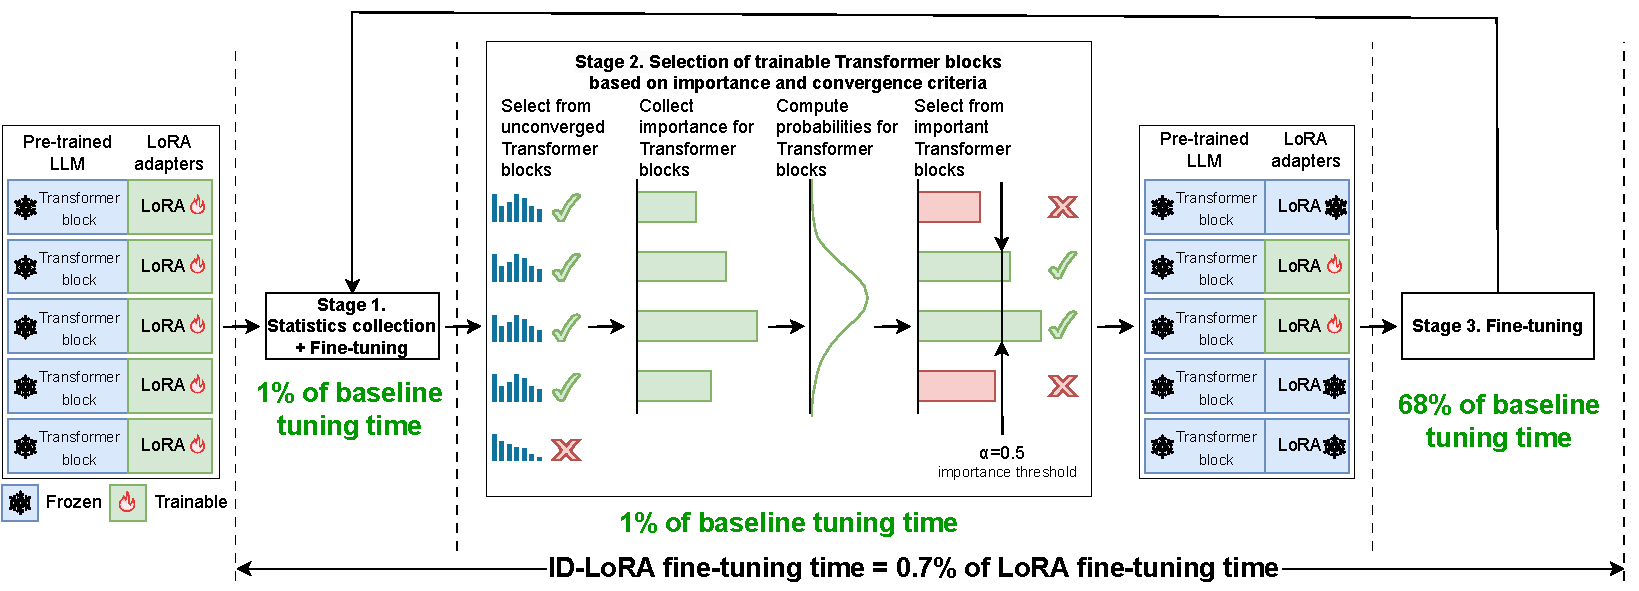
\includegraphics[width=0.99\textwidth]{sections/figures/id_lora.pdf}
        \caption{Key idea of proposed fine-tuning method: \ourmethodsFull{}.}
    \end{figure}
    Let \(h\) denote history defined as the number of steps to collect importance and convergence statistics, \(\alpha\) denote the ratio of Transformer blocks to be selected for fine-tuning.

    Initially, the fine-tuning process is divided into several periods, during which the algorithm switches the trainable Transformer
    blocks. Each \ourmethodshort{} period has 3 stages: statistics collection, selection of trainable Transformer blocks, and fine-tuning of the selected blocks. At the beginning of each stage, layer-wise importance statistic is collected during h steps. Next, algorithm determines unimportant Transformer blocks and removes them from the selection. After that, importance sampling of Transformer blocks is applied, and the ratio of the most important Transformer blocks (\(\alpha\)) is selected for further fine-tuning. At the same time, \lora{} \(A, B\) adapters for not-trainable Transformer blocks are merged up to the end of the fine-tuning. Merging non-updatable adapters allows to further accelerate the fine-tuning process and increase memory reduction. Obviously, with each training period, the number of trainable Transformer blocks diminishes. As a result, fine-tuning stops once there are no more trainable Transformer blocks. As an alternative or a complementary strategy to importance analysis, a convergence analysis was proposed by team to further reduce the number of trainable Transformer blocks. 

    The full \ourmethodshort{} method with importance analysis as my personal contribution and convergence analysis as team proposal is described in Algorithm 1.

    \begin{algorithm}
        \caption{\ourmethodshort{} (\(\alpha, h\))}
        \scriptsize
        \begin{algorithmic}[1]
            \State \(D\): fine-tuning dataset
            \State \(\mathcal{M}_{\Phi}\): pre-trained model
            \State \(\alpha\): trainable blocks selection ratio
            \State \(h\): number of accumulation steps
            \State 
            \State \(C\ \gets \{\} \): converged Transformer blocks 
            \State \(Q \gets \{\mathcal{M}_{\Phi}\} \): trainable Transformer blocks
            \State \(I \gets \{\}\): accumulated importance scores
            \State \(\mathcal{W} \gets \{\} \): accumulated layer weights
            \State \(use\_convergence=True\)
            \For{epoch \(i=1, \dots N\)}
                \For{train step \(i=1, \dots, K\), global batch \(b \in D\)}
                \State \(inp, labels \gets b\): data for forward
                \If{\(i < h\)}
                    \State \textbf{\{Statistics Collection + Fine-tuning Phase\}}
                    \For{layer \(\xi\) in \(\mathcal{M}_{\Phi}\)}
                        \State \(inp, out \gets forward(\xi, inp)\)
                        \State \(I \gets I \cup i(\xi, inp, out)\): calculate layer importance
                        \If{\(use\_convergence\)}
                            \State \(\mathcal{W} \gets \mathcal{W} \cup w_{\xi}\)
                        \EndIf
                        \State \(grads \gets backward(loss(out, labels))\)
                        \State \(apply\_gradients(grads)\)
                    \EndFor
                \ElsIf{\(i=h\)}
                    \State \textbf{\{Selection Phase\}}
                    \For{\(\mathcal{T}\) in \(Q\)}
                        \State \(I_\mathcal{T} \gets I(\{w_j: w_j \in \mathcal{T}\})\): aggregate importance of Transformer blocks (\ref{eq:aggregation})
                        \If{\(use\_convergence\)}
                            \State \(C_{\mathcal{T}} \gets c(\{w_i: w_i \in \mathcal{T}\})\): calculate layer convergence
                        \EndIf
                    \EndFor
                    \State \(T \gets \{\mathcal{T}_i \in Q: C_{\mathcal{T} \ge \varepsilon}\}\)
                    \State \(P \gets softmax(\{I_{\mathcal{T}}: t_{i} \in T\})\): select with (\ref{eq:probability})
                    \State \(T \gets \alpha * top\_p(Q, P)\): (\ref{eq:top-p-sampling})
                    \State \(Unfreeze(R)\)
                    \State \(Freeze(Q \setminus R)\)
                    \State \(Q \gets R\)
                \Else
                    \State \textbf{\{Fine-tuning Phase\}}
                    \State \(inp, out \gets forward(inp)\)
                    \State \(grads \gets backward(loss(out, labels))\)
                    \State \(apply\_gradients(grads)\)
                \EndIf
                \EndFor
            \EndFor
        \end{algorithmic}
    \end{algorithm}
    \subsection{Importance-based Transformer blocks selection}
        \paragraph{Statistics collection phase} The first step of \ourmethodshort{} is dedicated to statistics collection over several iterations of fine-tuning. During \(h\) steps, importance scores are accumulated for each layer of the model. As an importance estimation method several metrics have been considered, including Magnitude rule, Wanda rule, and Cosine Similarity rule. Notably, Magnitude \cite{han2016deepcompressioncompressingdeep} and Wanda \cite{wanda} importance rules are adapted to Transformer block importance estimation as described in Definition \ref{def:transformer-block-importance}.
        \begin{definition}\label{def:transformer-block-importance}
            Let \(T\) denote Transformer blocks, \(i_{\xi}\) denote importance score for \(\xi\) layer inside it, then importance of Transformer block is defined as:
            \begin{equation}\label{eq:aggregation}
                I(T) = \frac{\sum_{\xi \in T} i_{\xi}}{|T|}
            \end{equation}
        \end{definition}
        \paragraph{Selection phase} Upon reaching the \(h\) number of steps, the importance scores of each Transformer block are averaged. After that, the second step of \ourmethodshort{} begins, aimed at selecting important Transformer blocks. Based on the importance scores, selection probability for each Transformer block is computed (\ref{eq:probability}). Next, the Top-P sampling (\ref{eq:top-p-sampling}) is applied, which samples Transformer blocks with the highest probabili-ty scores until the sum of the scores reaches the specified threshold value. Then, the sampling probability for each Transformer block is recalculated (\ref{eq:probability}). Finally, \(\alpha\) of the most important Transformer blocks are selected for further fine-tuning. 
        \begin{equation}\label{eq:probability}
            P(T) = \frac{e^{I(T)}}{\sum_{k=1}^{\mathcal{M}_\Phi}e^{I(k)}},
        \end{equation}
        where \(I\) denotes Transformer block importance score.
        \begin{equation}\label{eq:top-p-sampling}
            Top_P = \{T_k \in \mathcal{M}_\Phi : \sum_{k=1}^{\mathcal{M}_\Phi}P(T_k)\le p\},
        \end{equation}
        where \(p\) denotes the threshold.
    \subsection{Convergence-based Transformer blocks selection}
    Besides the importance analysis, another solution proposed by the team is an optional convergence analysis, which identifies fully trained Transformer blocks that could be frozen, thereby further reducing the number of trainable Transformer blocks. Once per \(h\) steps, additional statistics for convergence analysis are accumulated.
    \begin{definition}\label{def:convergence-rule}
        Let \(\varepsilon\) denote convergence threshold, \(\hat{c}\) denote convergence metric. Then convergence rule for a layer is defined as:
        \begin{equation*}
            c(W_\xi) = 
            \begin{cases}
                1, & \hat{c}(W_\xi) < \varepsilon \\
                0, & \text{otherwise}
            \end{cases}
        \end{equation*}
    \end{definition}
    \begin{definition}\label{def:convergence-inequality}
        Transformer block T is converged if the following inequality with \\ convergence threshold \(\delta\) is satisfied: 
        \begin{equation}
            C(T) = \frac{\sum_{\xi \in T}c(W_{\xi})}{|T|} > \delta
        \end{equation}
    \end{definition}
    When statistic has been collected, the converged Transformer blocks are identified with with the help of convergence rule (\ref{def:convergence-rule}) and corresponding metrics (\ref{def:convergence-inequality}). After that, converged Transformer blocks are frozen up to the end of training, which leads to further reduction of the number of trainable parameters and an earlier stop of the fine-tuning process.
    \subsection{Key differences from existing approaches}
        \begin{itemize}
            \item Current approaches utilizes importance-based pruning of Transformer blocks on inference, introducing considerable quality degradation. In contrast, \ourmethodshort{} integrates the pruning process into the parameter-efficient fine-tuning with \lora{}, thereby preventing performance degradation.
            \item Prior methods incur extra computational costs by requiring inference on calibration data for importance estimation. Conversely, \ourmethodshort{} identifies essential Transformer blocks during the fine-tuning process without additional overhead and calibration data. 
            \item Current state-of-the-art approaches manually attach the \lora{} adapters to all Transformer blocks before the fine-tuning process. On the contrary, \ourmethodshort{} offers an innovative approach that enables automatic assignment of \lora{} \(A, B\) adapters only to important Transformer blocks. 
            \item \ourmethodshort{} applies the idea of additional convergence analysis to further reduce the number of trainable Transformer blocks.
        \end{itemize}

    \section*{Chapter 3. Evaluation of the proposed method}
\addcontentsline{toc}{section}{Chapter 3. Evaluation of the proposed method}
\setcounter{section}{3}
\setcounter{subsection}{0}
To assess the feasibility of the \ourmethodshort{}, comprehensive evaluation of the proposed solution has been applied with detailed results being presented in the article \cite{Demidovskij2025}. 

\subsection{Software implementation}
    The software implementation is made in a form of Python package, adhering to the principles of object-oriented programming, and is fully compatible with all the considered \llms{}. The code is the intellectual property of Huawei and cannot be disclosed in this work.

\subsection{Protocol}\label{subsec:protocol}
For the evaluation purposes, six \llms{} with different numbers of parameters were chosen to estimate the performance on different scales of \llms{}: 
\begin{itemize}
    \item \gpt{} (24 Transformer blocks);
    \item \llamaTwoSmall{} (32 Transformer blocks);
    \item \llamaTwoBig{} (40 Transformer blocks);
    \item \qwenSmall{} (36 Transformer blocks);
    \item \qwenMedium{} (28 Transformer blocks);
    \item \qwenLarge{} (64 Transformer blocks).
\end{itemize}
The \gpt{} model was taken from \textit{transformers v4.33.2},  \llamaTwoSmall{}, \llamaTwoBig{}, \qwenSmall{}, \qwenMedium{}, \qwenLarge{} models were taken from HuggingFace hub \cite{huggingface:llama2-7b}, \cite{huggingface:llama2-13b}, \cite{huggingface:qwen-small}, \cite{huggingface:qwen-medium}, \cite{huggingface:qwen-large}.

\begin{table}[H]
    \caption{Training hardware used for the evaluation of considered approaches.}
    \centering 
    \scriptsize
    \begin{tabularx}{0.99\textwidth}{M|x|x}
    \toprule
    & 
    \bfseries \gpt{} & 
    \bfseries \llamaTwoSmall{}, \llamaTwoBig{}, \qwenSmall{}, \qwenMedium{}, \qwenLarge{} \\
    \midrule
    % \bottomrule
    CPU & CPU 32 cores with 3.0GHz & CPU 32 cores with 2.90GHz \\ 
    \midrule
    OS & Ubuntu 20.04.6 LTS & Ubuntu 20.04.04 LTS \\
    \midrule
    Driver Version & 515.43.04 & 535.183.01 \\
    \midrule
    Kernel Version & 5.4.0-176-generic & 5.15.0-125-generic \\
    \midrule
    CUDA Toolkit Version & 11.7.64 & 12.2 \\
    \midrule
    Training Libraries & \textit{transformers} 4.33.0,  \textit{PyTorch} 2.1.0, \textit{DeepSpeed} 0.15.4, \textit{peft} v.0.18.0 & \textit{transformers} 4.45.0,  \textit{PyTorch} 2.1.0, \textit{DeepSpeed} 0.15.4, \textit{peft} v.0.18.0 \\
    \bottomrule
\end{tabularx}
\label{tab:hardware}
\end{table}

\begin{table}[H]
    \caption{Training protocol used for the evaluation of considered approaches.}
    \centering 
    \footnotesize
    \renewcommand{\arraystretch}{0.5}
    \begin{tabularx}{0.99\textwidth}{M|x|x}
    \toprule
    & 
    \bfseries \gpt{} & 
    \bfseries \llamaTwoSmall{}, \llamaTwoBig{}, \qwenSmall{}, \qwenMedium{}, \qwenLarge{} \\
    \midrule
    Sequence Length & 512 & 256 \\ 
    \midrule
    Learning Rate & 6e-4 & 1e-5 \\
    \midrule
    AdamW $\beta_1$ & 0.9 & 0.9 \\
    \midrule
    AdamW $\beta_2$ & 0.99 & 0.99 \\
    \midrule
    Weight Decay & 0.01 & 0 \\
    \midrule
    Epochs & 2 & 2 \\
    \midrule
    Precision & fp16 & bf16 \\
    \midrule
    \lora{} $r$ & 16 & 16 \\
    \midrule
    \lora{} $\alpha$ & 32 &  32\\
    \midrule
    Ratio of Transformer blocks & 0.8 &  0.6\\
    \bottomrule
\end{tabularx}
\label{tab:training_protocol}
\end{table}

Since \lora{} is the de-facto standard approach for fine-tuning acceleration, it was selected as a baseline for computational experiments on quality and acceleration. In addition, the most prominent modifications of \lora{}, such as \dora{} \cite{dora}, \pissa{} \cite{pissa}, \adalora{} \cite{adalora} were chosen as reference methods during the evaluation. The implementation of these approaches was taken from the \textit{peft v.0.18.0} library \cite{peft}.

Used training hardware and software are described in Table \ref{tab:hardware}. Training protocol for each model is described in Table \ref{tab:training_protocol}. The \textit{Ratio of Transformer blocks} row means the ratio of Transformer blocks selected for fine-tuning with chosen approaches. Notably, the \gpt{} model requires a higher number of updated layers than all other models, because a greater number of layers in the model allows for a smaller amount of updated layers, since a substantial proportion of the layers will still be updated.

After the fine-tuning, in order to estimate the final quality of the model, zero-shot accuracy was measured on commonsense reasoning datasets: PIQA \cite{piqa}, HellaSwag \cite{hellaswag}, Winogrande \cite{winogrande}, ARC \cite{arc}, OpenbookQA \cite{openbookqa}, MMLU \cite{mmlu} using the lm-evaluation-harness package \cite{lm_eval}. Zero-shot PPL was measured on language modelling dataset WikiText2 \cite{wikitext}. In this work, an average accuracy and perplexity are presented. The detailed results for each of these datasets are presented in the paper \cite{Demidovskij2025}.
\begin{table}[!t]
    \caption{Quality results after the fine-tuning with considered approaches on \gpt{}, \llamaTwoSmall{}, and \llamaTwoBig{}.}
    \centering  
    \scriptsize
    \begin{tabularx}{0.99\textwidth}{AM|TTT}

        \toprule

        \bfseries Model &
        \bfseries Method & 
        \bfseries Average accuracy, \(\uparrow\) & 
        \bfseries Perplexity, \(\downarrow\) &
        \bfseries Acceleration, \(\uparrow\) \\

        \midrule 
        \multirow{11}{*}{\gpt{}}
        & \lora{} (baseline) & 37.5 & 173.1 & -- \\
        \cmidrule{2-5}
        & \dora{} & 37.0 & 184.2 & -21.6 \\
        & \pissa{} & 34.9 & 172.1 & 0.9 \\
        & \adalora{} & 36.9 & 179.2 & -1.3 \\
        \cmidrule{2-5}
        & \uidl{} & 37.9 & 173.8 & -39.5 \\
        & \lisa{} & \bfseries 40.8 & 205.7 & -40.9 \\
        & \ows{} & 31.3 & 180.2 & -61.3 \\
        & \sleb{} & 36.3 & 450.1 & 13.5 \\
        & \shortllama{} & 33.1 & 400.5 & 12.6 \\
        \cmidrule{2-5}
        & \cellcolor{DarkOliveGreen3} \ourmethodshort{} & \cellcolor{DarkOliveGreen3} 38.0 & \cellcolor{DarkOliveGreen3} \bfseries 72.7 & \cellcolor{DarkOliveGreen3} \bfseries 25.2 \\
        \midrule
        \multirow{9}{*}{\llamaTwoSmall{}}
        & \lora{} (baseline) & 59.9 & \bfseries 9.2 & -- \\
        \cmidrule{2-5}
        & \dora{} & 59.8 & \bfseries 9.2 & -407.3 \\
        & \pissa{} & \bfseries 60.9 & 9.4 & 1.7 \\
        & \adalora{} & 59.3 & \bfseries 9.2 & -51.6 \\
        \cmidrule{2-5}
        & \uidl{} & 59.3 & \bfseries 9.2 & -31.2 \\
        & \sleb{} & 42.7 & 403.6 & -11.0 \\
        & \shortllama{} & 41.1 & 53.1 & 13.4 \\
        \cmidrule{2-5}
        & \cellcolor{DarkOliveGreen3} \ourmethodshort{} & \cellcolor{DarkOliveGreen3} 59.4 & \cellcolor{DarkOliveGreen3} \bfseries 9.2 & \cellcolor{DarkOliveGreen3} \bfseries 29.2 \\
        \midrule
        \multirow{9}{*}{\llamaTwoBig{}}
        & \lora{} (baseline) & 63.8 & \bfseries 7.7 & -- \\
        \cmidrule{2-5}
        & \dora{} & 63.7 & \bfseries 7.7 & -203.3 \\
        & \pissa{} & \bfseries 64.5 & 7.9 & -0.3 \\
        & \adalora{} & 63.1 & \bfseries 7.7 & -92.9 \\
        \cmidrule{2-5}
        & \uidl{} & 63.6 & \bfseries 7.7 & -22.7 \\
        & \sleb{} & 49.8 & 20.0 & -70.0 \\
        & \shortllama{} & 42.4 & 72.8 & -110.7 \\
        \cmidrule{2-5}
        & \cellcolor{DarkOliveGreen3} \ourmethodshort{} & \cellcolor{DarkOliveGreen3} 63.6 & \cellcolor{DarkOliveGreen3} \bfseries 7.7 & \cellcolor{DarkOliveGreen3} \bfseries 44.8 \\
        \midrule
        \multirow{9}{*}{\qwenSmall{}}
        & \lora{} (baseline) & 62.9 & 15.5 & -- \\
        \cmidrule{2-5}
        & \dora{} & 62.9 & 15.3 & -201.0 \\
        & \pissa{} & \bfseries 63.5 & \bfseries 11.8 & -0.6 \\
        & \adalora{} & 62.3 & 15.1 & -71.5 \\
        \cmidrule{2-5}
        & \uidl{} & 62.7 & 15.5 & -20.1 \\
        & \sleb{} & 44.5 & 77.4 & -30.4 \\
        & \shortllama{} & 15.1 & 72.8 & 0.1 \\
        \cmidrule{2-5}
        & \cellcolor{DarkOliveGreen3} \ourmethodshort{} & \cellcolor{DarkOliveGreen3} 62.9 & \cellcolor{DarkOliveGreen3} 15.5 & \cellcolor{DarkOliveGreen3} \bfseries 28.6 \\
        \midrule
    \end{tabularx}
    \label{tab:quality_1}
\end{table}
\subsection{Analysis of the obtained results}
Computational experiments with chosen models and approaches are presented in Table \ref{tab:quality_1}. For \qwenLarge{} model, the evaluation of \dora{} approach was not presented, as memory requirements did not fit to used hardware.

\ourmethodshort{} provides an average acceleration of 33.1\%
with a considerable maximum speedup of 44.8\% for \llamaTwoBig{}
with a quality decrease of less than 0.2\%.  In addition, \ourmethodshort{} significantly outperforms \pissa{}, \dora{}, and \adalora{} from the point of acceleration, and provides 0.4\% of quality improvement compared to \textit{\adalora{}} and comparable performance to \textit{\dora{}}. However, it leads 0.2\% quality decrease compared to \pissa{} as \pissa{} employs an SVD initialization
of \lora{} \(A, B\) adapters, which provides them with the most important information from the original weights \(W\).

\subsection{Sensitivity analysis}
    Sensitivity analysis of \(\alpha\) and \(h\) hyperparameters of \ourmethodshort{} and importance metrics is presented in Figure \ref{fig:ablation_alpha}, Figure \ref{fig:ablation_h}, and Figure \ref{fig:ablation_importance}. They were analyzed in terms of their impact on the resulting quality and acceleration.
    \subsubsection{Analysis of hyperparameter \(\alpha\)}
        \begin{figure}[H]
            \centering
            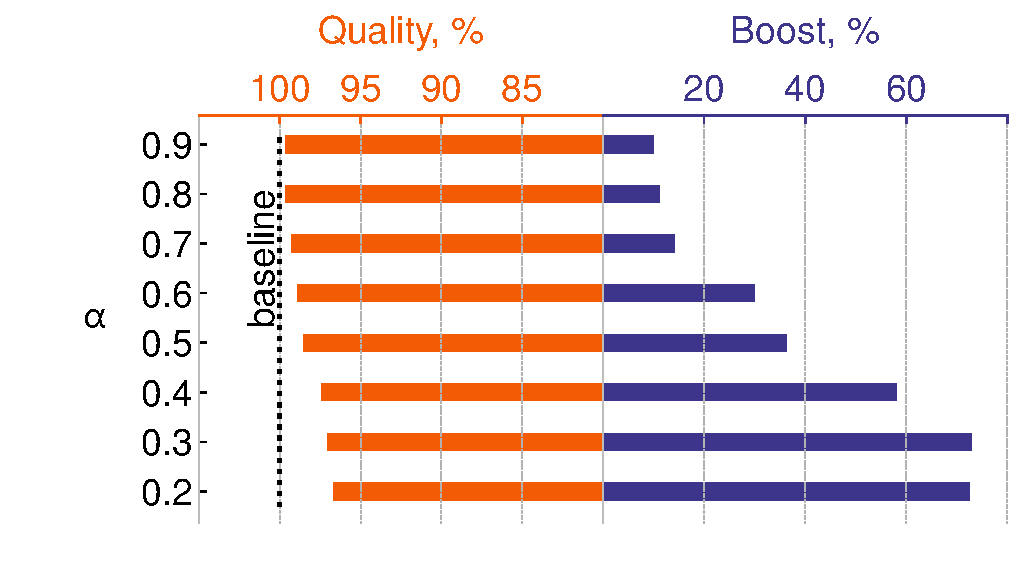
\includegraphics[width=0.6\textwidth]{sections/figures/ablation_alpha.pdf}
            \caption{Sensitivity analysis of \ourmethodshort{} to the \(\alpha\) hyperparameter. \(h\) is 10, importance metric is cosine similarity.}
            \label{fig:ablation_alpha}
        \end{figure}
        Ablation study of the \(\alpha\) hyperparameter of
        \ourmethodshort{} is presented in Figure \ref{fig:ablation_alpha}. Obtained results demonstrate that increasing \(\alpha\) significantly affects both acceleration and model quality. In particular, a maximum speedup of 72.6\% is observed at \(\alpha\) = 0.2, where only 20\% of the Transformer blocks are trained. However, it leads to a 3.3\% increase in perplexity, suggesting underfitting. Minimal quality degradation (0.3\%) occurs at higher \(\alpha\) values (0.8 and 0.9), where 80-90\% of the Transformer blocks are trained initially. \(\alpha\) = 0.6 is identified as the optimal setting for balancing speed and quality. 
    \subsubsection{Analysis of hyperparameter \(h\)}
        \begin{figure}[H]
            \centering
            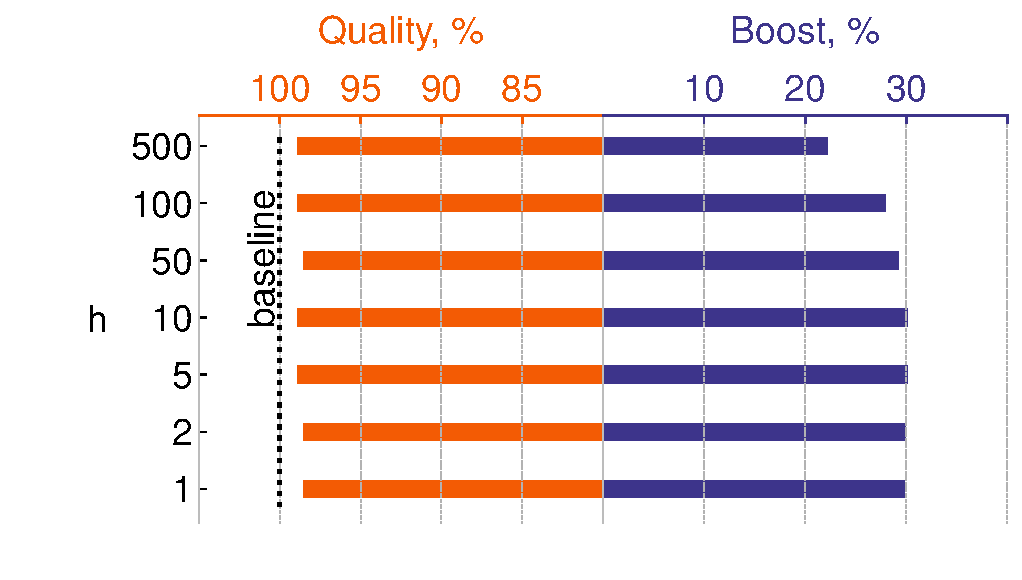
\includegraphics[width=0.6\textwidth]{sections/figures/ablation_h.pdf}
            \caption{Sensitivity analysis of \ourmethodshort{} to the \(h\) hyperparameter. \(\alpha\) is 0.6, importance metric is cosine similarity.}
            \label{fig:ablation_h}
        \end{figure}
        Ablation study of the \(h\) hyperparameter of
        \ourmethodshort{} is presented in Figure \ref{fig:ablation_h}. According to the achieved results, variations in hyperparameter \(h\) do not significantly impact quality, with only a 0.3\% change in perplexity was observed between \(h\) = 1 and \(h\) = 500. The smallest \(h\) value accelerates fine-tuning by 29.8\%, indicating that even a single training step can adequately capture the importance of a Transformer block. This observation is supported by the relative stability of model quality across different \(h\) settings, as shown in Figure \ref{fig:ablation_h}. \(h\) = 10 is identified as the optimal setting for balancing speed and quality. 
    \subsubsection{Analysis of importance metrics}
        \begin{figure}[H]
            \centering
            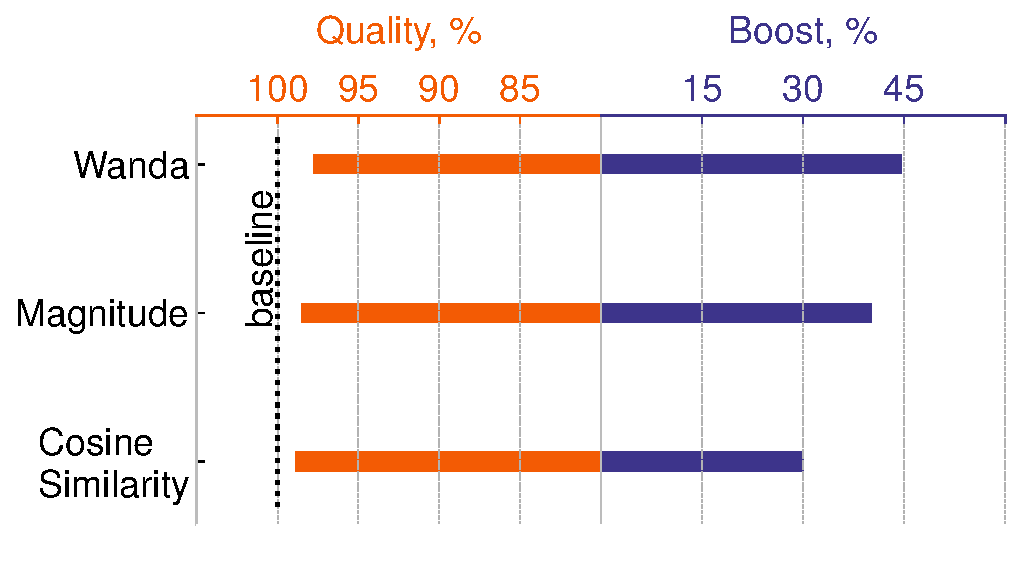
\includegraphics[width=0.6\textwidth]{sections/figures/ablation_importance.pdf}
            \caption{Sensitivity analysis of \ourmethodshort{} to considered importance metrics. \(\alpha\) is 0.6, \(h\) is 10.}
            \label{fig:ablation_importance}
        \end{figure}
         An ablation study of importance metrics is presented in Figure \ref{fig:ablation_importance}. 
         Despite the fact, that cosine similarity is considered an optimal choice, an additional ablation study on applying standard pruning metrics, such as Magnitude (\ref{eq:magnitude}) and Wanda (\(\ref{eq:wanda}\)) was performed. Notably, Magnitude and Wanda importance metrics are adapted to Transformer block importance estimation as described in Definition \ref{def:transformer-block-importance}.
        \begin{definition}\label{def:transformer-block-importance}
            Let \(T\) denote Transformer blocks, \(i_{\xi}\) denote importance score for \(\xi\) layer inside it, then importance of Transformer block is defined as:
            \begin{equation}\label{eq:aggregation}
                I(T) = \frac{\sum_{\xi \in T} i_{\xi}}{|T|}
            \end{equation}
        \end{definition}
        Sensitivity analysis reveals that the Magnitude metric yields the best balance between acceleration and quality. In contrast, the Wanda metric, despite considering input activations, provides a higher speedup at the
        cost of increased quality degradation by 2\% compared to the baseline. Although cosine similarity decelerates the fine-tuning on 7\% compared with the Magnitude, it degrades model quality the least, representing the most suitable choice, as minimizing the drop in model quality is particularly crucial in the context of importance-based fine-tuning. This conclusion is also consistent with the results of last year's study.
    \subsection{Summary}
        In conclusion, the quality and acceleration of the proposed \ourmethodshort{} was estimated across different \llm{} scales (350M, 3B, 7B, 13B, 32B) and a broad range of tasks. According to the obtained results, \ourmethodshort{} significantly outperforms the baseline \lora{} approach and reference \dora{}, \pissa{}, and \adalora{} methods from the point of acceleration. \ourmethodshort{} provides on average 33\% of fine-tuning time speedup compared to \lora{} approach. Moreover, \ourmethodshort{} achieves near-lossless performance with an average quality degradation of 0.2\% compared to baseline \lora{} approach. 
        
        According to the conducted ablation study, the hyperparameter \(\alpha=0.6\) and hyperparameter \(h=10\) are considered an optimal choice with importance metric being cosine similarity. 

    \section*{Conclusion}
\addcontentsline{toc}{section}{\protect\numberline{}Conclusion}

This study was aimed to provide an in-depth examination of existing importance estimation techniques across various scenarios, with a particular focus on the impor-tance estimation of Transformer blocks to optimize the fine-tuning process.

Throughout the research, the concept of "importance" was defined as the identifi-cation of structures that can be removed without significantly affecting model performance. In particular, four types of structures withing \llm{} could be estimated with the impor-tance.

\begin{itemize}
\item \textbf{Separate Weights}: In \llms{} certain weights act as "systematic outliers" \\ significantly deviating from the average of their distribution and susbtantially affecting model performance. 
\item \textbf{Layers}: In \llms{} not all layers are of equal importance. Some layers exhibit a high level of redundancy, particularly within Multi-Head Attention module, while MLP layers are crucial for maintaining the overall effectiveness of the model.
\item \textbf{Transformer blocks}: In \llms{} Transformer blocks have varying levels of redundancy, especially in middle or later layers, with initial and final layers being more critical.
\item \textbf{Generated Architectures}: While designing Transformer models automatically, performance of predicted architectures could be estimated with importance heuristics, that approximates the model performance. 
\end{itemize}

After a comprehensive overview, several key challenges in the field of importance estimation were identified:
\begin{enumerate}
    \item \textbf{Lack of a Unified Methodology}: There is no general importance heuristic applicable across different scenarios and various contexts.
    \item \textbf{Quality Degradation}: Existing solutions often reduce computational costs but at the expense of model quality, which can degrade by at least 1-2\% or completely compromise the language modeling capabilities of \llms{}.
    \item \textbf{Computational Costs}: Most importance-based methods require extensive addi-tional inference on calibration data, significantly increasing time overhead.
\end{enumerate}

In the second part of this study, comparative analysis of existing approaches for evaluating the importance of Transformer blocks within LLMs during the fine-tuning process was conducted. This analysis not only assessed current techniques but also sought to optimize fine-tuning by selectively updating essential Transformer blocks. Key Transformer blocks-based importance approaches like \uidl{}, \ows{}, \sleb{}, \\ \shortllama{} were evaluated. As a baseline a cutting-edge \lora{} approach has been used. As reference methods the \lisa{} approach and the most prominent modifications of \lora{} -- \dora{}, \pissa{}, and \adalora{} -- were estimated. 

The 6 models fine-tuning was estimated with considered approaches, including \gpt{}, \llamaTwoSmall{}, \llamaTwoBig{}, \qwenSmall{}, \qwenMedium{}, and \qwenLarge{}. After the fine-tuning, in order to estimate the final quality of the model, zero-shot accuracy was measured on commonsense reasoning datasets: PIQA \cite{piqa}, HellaSwag \cite{hellaswag}, Winogrande \cite{winogrande}, ARC \cite{arc}, OpenbookQA \cite{openbookqa}, MMLU \cite{mmlu} using the lm-evaluation-harness package \cite{lm_eval}. Zero-shot PPL was measured on language modelling dataset WikiText2 \cite{wikitext}.

The results showed that:
\begin{itemize}
\item The \uidl{} method is the preferred option when quality maintenance is para-mount as this approach demonstrated robust performance improvements with fewer Transformer blocks than \lora{}. However, \uidl{} did not accelerate the process due to the required additional inference.
\item For scenarios where speed is prioritized over certain quality loss, the \sleb{} and \shortllama{} methods are effective as these approaches provide a 38\% reduction in fine-tuning time.
\item The \lisa{} approach is suitable when there are ample resources available for full parameter updates as it is able to accelerate the full fine-tuning process while maintaining the performance.
\end{itemize}

Given these findings, existing methods for estimating the importance of Transfor-mer blocks have potential for enhancing the fine-tuning process by updating only the essential units. However, there exist several limitations, that needs to be solved. First, enable the removal of non-essential units without degrading model quality. Second, efficiently pinpoint essential Transformer blocks without incurring additional time costs. Third, employ a general methodology that aligns well with overall model performance and could be applicable to various scenarios.


Therefore, future directions of this study within research project in Huawei include:
\begin{enumerate}
\item Develop a general importance estimation methodology that performs well across various scenarios and structures.
\item Create an importance estimation approach that efficiently identifies essential Transformer blocks without incurring additional time costs and without degra-ding performance.
\item Conduct a comparative analysis of other importance estimation techniques for weights, layers, and architectures.
\item Optimize the state-of-the-art \lora{} approach by automatically assigning \lora{} A,B adapters only to essential Transformer blocks, significantly reducing fine-tuning time while maintaining accuracy.
\end{enumerate}

\addcontentsline{toc}{section}{Reference List}
\nocite{*}
% \bibliographystyle{ref/IEEEannot}
% \bibliography{ref/annot}
\printbibliography
\end{document}